\section{Codebase}\label{sec:code}

As a baseline we used the libDAI library \cite{Mooij_libDAI_10} which provides an implementation for loopy belief propagation using the max residual updating scheme. With the library, it was simple to implement the recommendation system as proposed in \cite{Ha:2012:TRT:2396761.2398636}.

\mypar{Code structure}
Figure \ref{overviewflow} shows a high-level overview of the code structure. After an initialization phase the BP algorithm is invoked which loops until a specified maximum number of iterations is reached, the maximum residual becomes zero or the change in the updated messages is smaller than some specified tolerance. In every iteration, findMaxResidual is called to determine the message that should be updated next (by updateMessage). The actual update step goes quickly, because it only assigns newMessage to message. The costly part of the algorithm is the re-computation of newMessage for all neighbouring nodes that are affected by the change. To do so, calcNewMessage is called for every candidate, which first computes a product over all incoming messages (calcIncomingMessageProduct) and then marginalizes this product of messages over all other variables (marginalizeProductOntoMessage). Note that the residual is simply $||\mathtt{message}-\mathtt{newMessage}||_\infty$. 

%\lstset{basicstyle=\tiny\ttfamily}
%\begin{table}
%\begin{lstlisting}
%init()
%while (not done)
%   messageToUpdate <-- findMaxResidual;
%\end{lstlisting}
%\caption{Pseudo code for Residual BP}
%\end{table}

The methods that get called the most often are updateResidual, calcIncomingMessageProduct and marginalizeProductMessage. Hence, our optimizations will mostly focus on these.

\begin{figure}\centering
    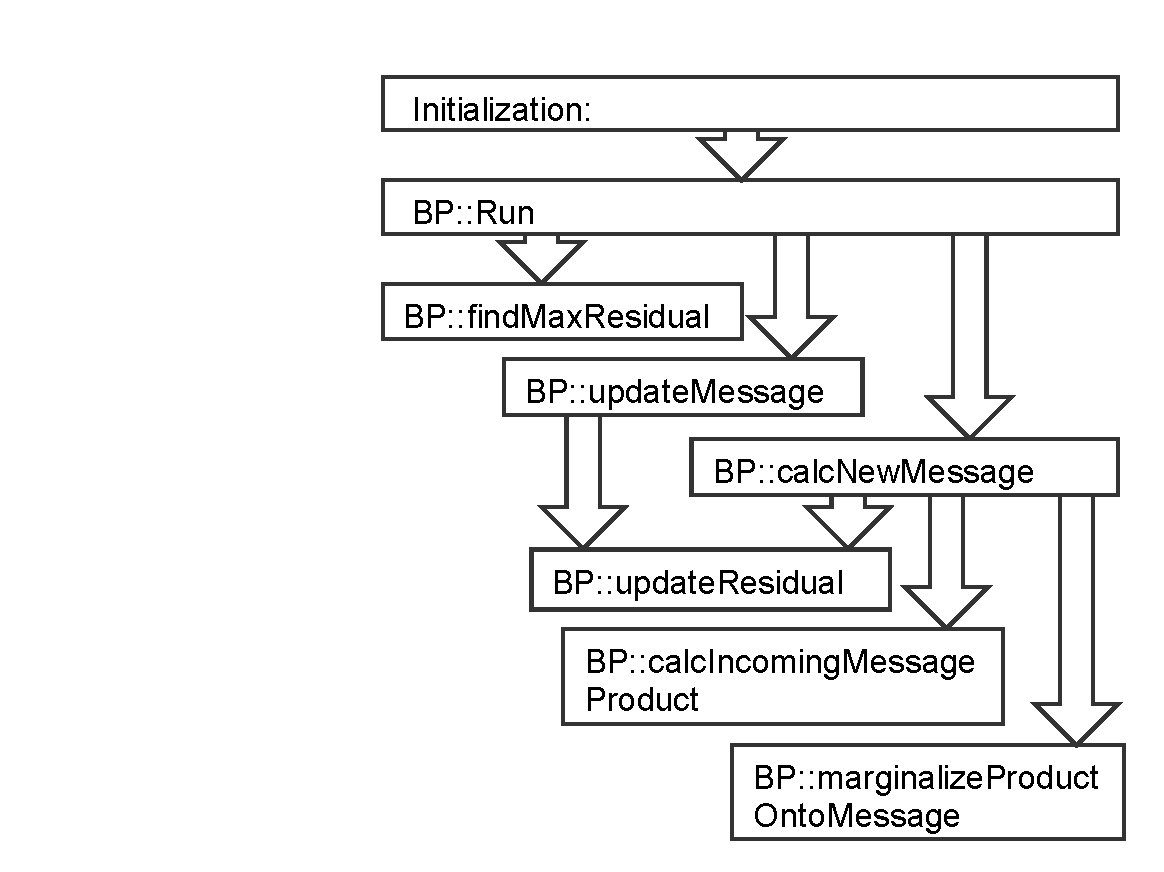
\includegraphics[scale=0.5, trim={6.45cm 0cm 0 1.25cm},clip]{graphics/loopybp-compact.pdf}
  \caption{Flow (top to bottom) of our program. Arrows denote that a methods gets called from an other, BP is the namespace used for all functions that deal with belief propagation.\label{overviewflow}}
\end{figure}

